\chapter{Design}
\label{ch:5}

In this chapter, I will design a system that will fulfil user requirements described in Chapter~\ref{ch:4}.

\section{The Idea}
\label{sec:idea}

As was mentioned in Chapter \ref{ch:1}, the system will implement the methodology from the journal \cite{roig2013retail}. It will be responsible for guiding users through the site selection process if it was conducted manually, but without requiring users to dive into all the technical details.

The system defines the following steps for the user to achieve the results (Figure \ref{fig:system-process-diagram}).

\begin{figure}[ht]\centering
  \centering
  \includesvg[width=1\linewidth]{obrazky-figures/ch5/system-process-diagram.svg}
  \caption{System process diagram.}
  \label{fig:system-process-diagram}
\end{figure}

\subsection{Selecting Possible Sites}

The methodology outlines two key concepts: Geo-demand and Geo-competition, both of which were described in Chapter \ref{ch:2}. These concepts help to identify areas where there is a demand for a certain type of business, but it's currently lacking. Using a dataset with a number of people living at specific addresses, it becomes possible for the system to identify geo-demand automatically. Something similar is possible to do with geo-competition: the dataset for geo-demand and another one with real outlets and their square areas are going to serve as input for the Huff model to identify trading areas.

Once these concepts are identified, the system can apply kernel density estimation on both geo-demand and geo-competition. Then, by combining these concepts together, it becomes possible to identify areas where many people are not provided with the services of a business. The system will display this information as a heatmap layer, making it easy for the user to select potential locations.

\subsection{Define Location Attributes}

Once potential sites are selected, the next step requires the user to input location attributes, such as visibility, distance to competition or anything else that can described using quantitative or qualitative information. The information itself must be provided by the user as well.

\subsection{Compare Location Attributes}

When the user has defined the attributes, in the next step, he has to estimate them on a scale of 1 to 9, which is then used as input for the AHP method.

\subsection{Result}

The AHP method will output the list of potential sites that will contain ratings calculated based on the user's input.

\section{System Architecture}
\label{section:architecture}

The system for informed decisions in the site selection process will be developed as a full-stack web application (Figure \ref{fig:system-architecture}).

\begin{figure}[ht]\centering
  \centering
  \includesvg[width=0.7\linewidth]{obrazky-figures/ch5/system-architecture.svg}
  \caption{System architecture}
  \label{fig:system-architecture}
\end{figure}

\textbf{User} represents an individual that needs to utilize this system and its site selection process. All the user's actions are controlled by the client. The client meanwhile communicates with the configured server to handle certain regions on a map and to evaluate input provided by a user from the client.

\textbf{Admin} is an individual who configures the server with the region and related datasets. Both individuals can be the same person.

\subsection{Front-End Architecture}
\label{implementation:front-end}

The front-end should allow users to interact with spatial data and provide user inputs. It will have a dynamic map displaying various data layers and components presenting information relevant to each stage of the decision-making process, such as possible location selection, site attributes definition etc.

\subsubsection{Process Control}
\label{subsec:processControl}

Each step of the process will be managed client-side rather than on the server. This approach is deliberate because there is no need to store user-related data, sessions, or other sensitive information on the back-end. Instead, the back-end primarily handles pre-defined data utilized by these client-side processes.

\subsubsection{Abstractions}

The client application will contain several crucial abstractions for the functionality of the system: Marker, Attribute and Map. All of them will be described in Chapter \ref{ch:6}.

\subsection{Back-End Architecture}

The back-end will serve as the central engine driving the system, offering a way to configure and adapt to different cities and datasets associated with specific categories of products. This flexibility enables the creation of multiple instances of the application for diverse cities and product categories defined within the back-end.

\subsubsection{Configuration}
\label{subsec:configuration}

Utilizing configuration information, the server can set up map positions and estimate potential high-demand areas based on the type of business and datasets provided by the user.

In order to analyze data by the system, the datasets will have to follow a certain format. For this reason, a user who sets the system up will have to use some parsing tool to convert the original dataset into the required one. This process will be described in detail in section \ref{sec:testingApplicationWithRealData}.

\subsubsection{Endpoints}

To provide all the functionalities, the back-end will expose various endpoints accessible for specific actions, each triggered at distinct stages controlled by the clients.

\section{UI Prototypes}

The core component is a map. It allows users to interact with the system and control the entire flow of the decision-making process. The map will provide retailers with useful insights for the area based on their input that can be analyzed. Another important component will be a modal window where the user can configure the importance of location attributes. The design also presents prototypes of the system's main components.

\subsection{Map}

The central hub of the system is the map page, it is expected to be the most frequently accessed feature (Figure \ref{fig:map-prototype}). This page contains various components, such as a menu, a panel with location information and controls to work with the map. The sidebar menu includes a toolkit, offering users a range of tools to manipulate and engage with data, for example they can explore data layers.

Moreover, an informative panel is integrated into the left corner of a map, presenting location attributes for users to analyze and make comparisons. This feature enhances the user's ability to obtain insights from the data presented on the map.

Additionally, the map serves as a dynamic platform where all procedure steps are executed and visually represented. To guide users through each step, hints are placed, providing informative cues and a smooth navigation experience. This comprehensive approach ensures that non-technical users can effortlessly engage with the system, analyze data, and make informed decisions with ease.


\subsection{User Inputs}

This module acquires user input in the form of a rating ranging from 1 to 9. This rating reflects the assessment of specific attributes related to potential locations. The purpose is to customize the behaviour of a procedure based on individual user preferences and evaluations (Figure \ref{fig:location-attributes}). Input windows like this will pop up on the page with an interactive map during certain steps of a process. Users will be able to manually open them and rerun location evaluation if needed.

\begin{figure}[ht]\centering
  \centering
  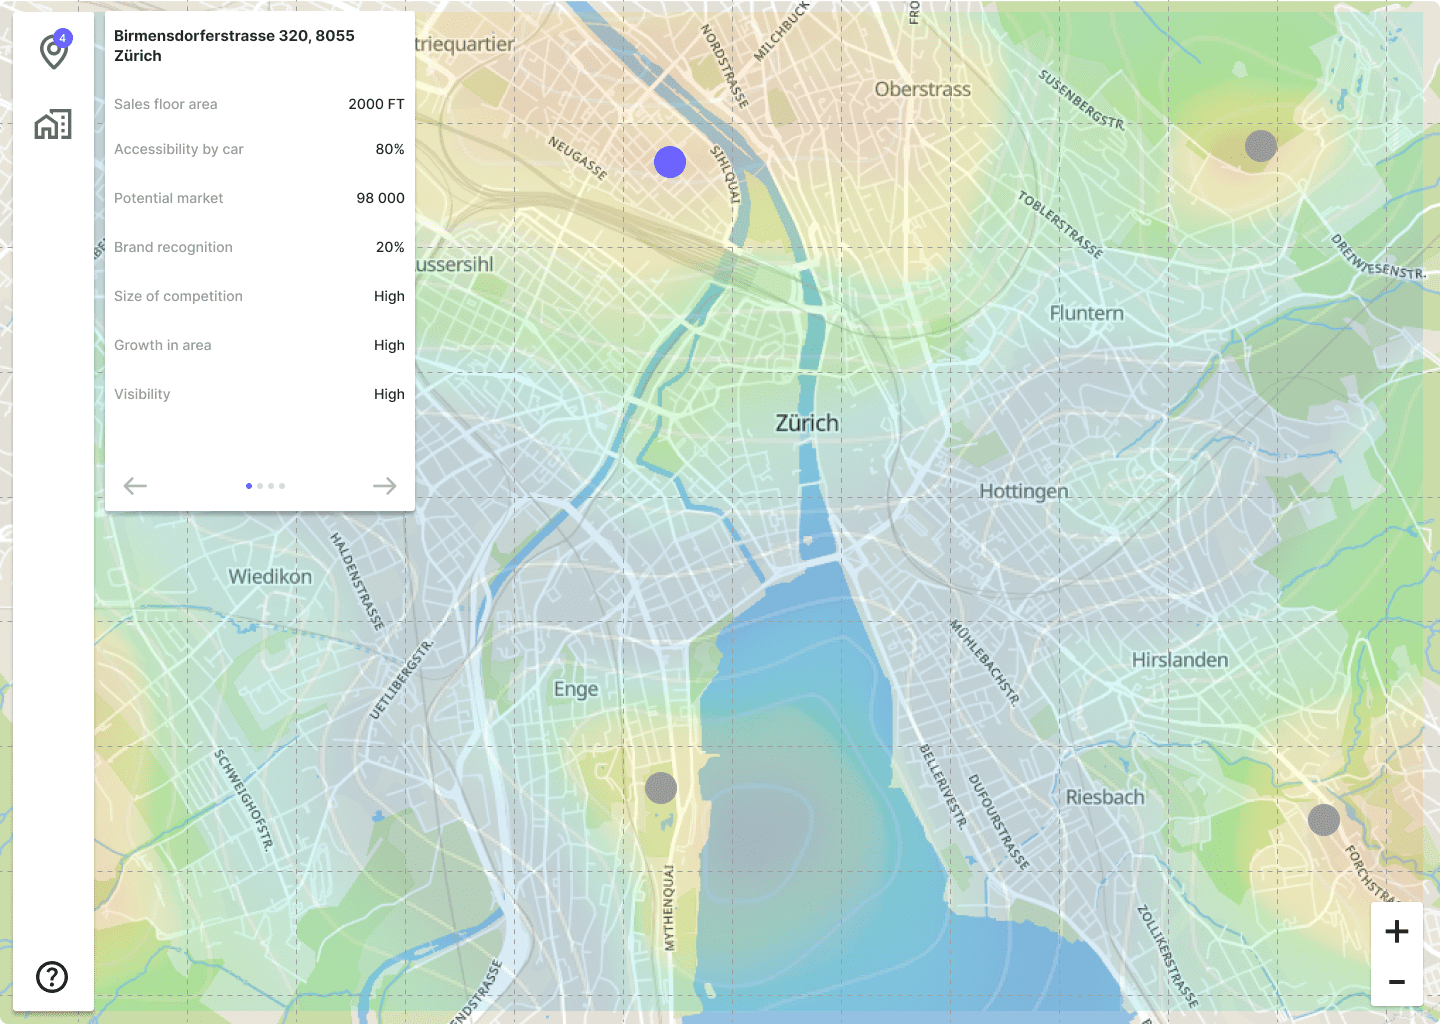
\includegraphics[width=0.9\linewidth]{obrazky-figures/ch5/map.png}
  \caption{Prototype of a map component.}
  \label{fig:map-prototype}
\end{figure}

\begin{figure}[ht]\centering
  \centering
  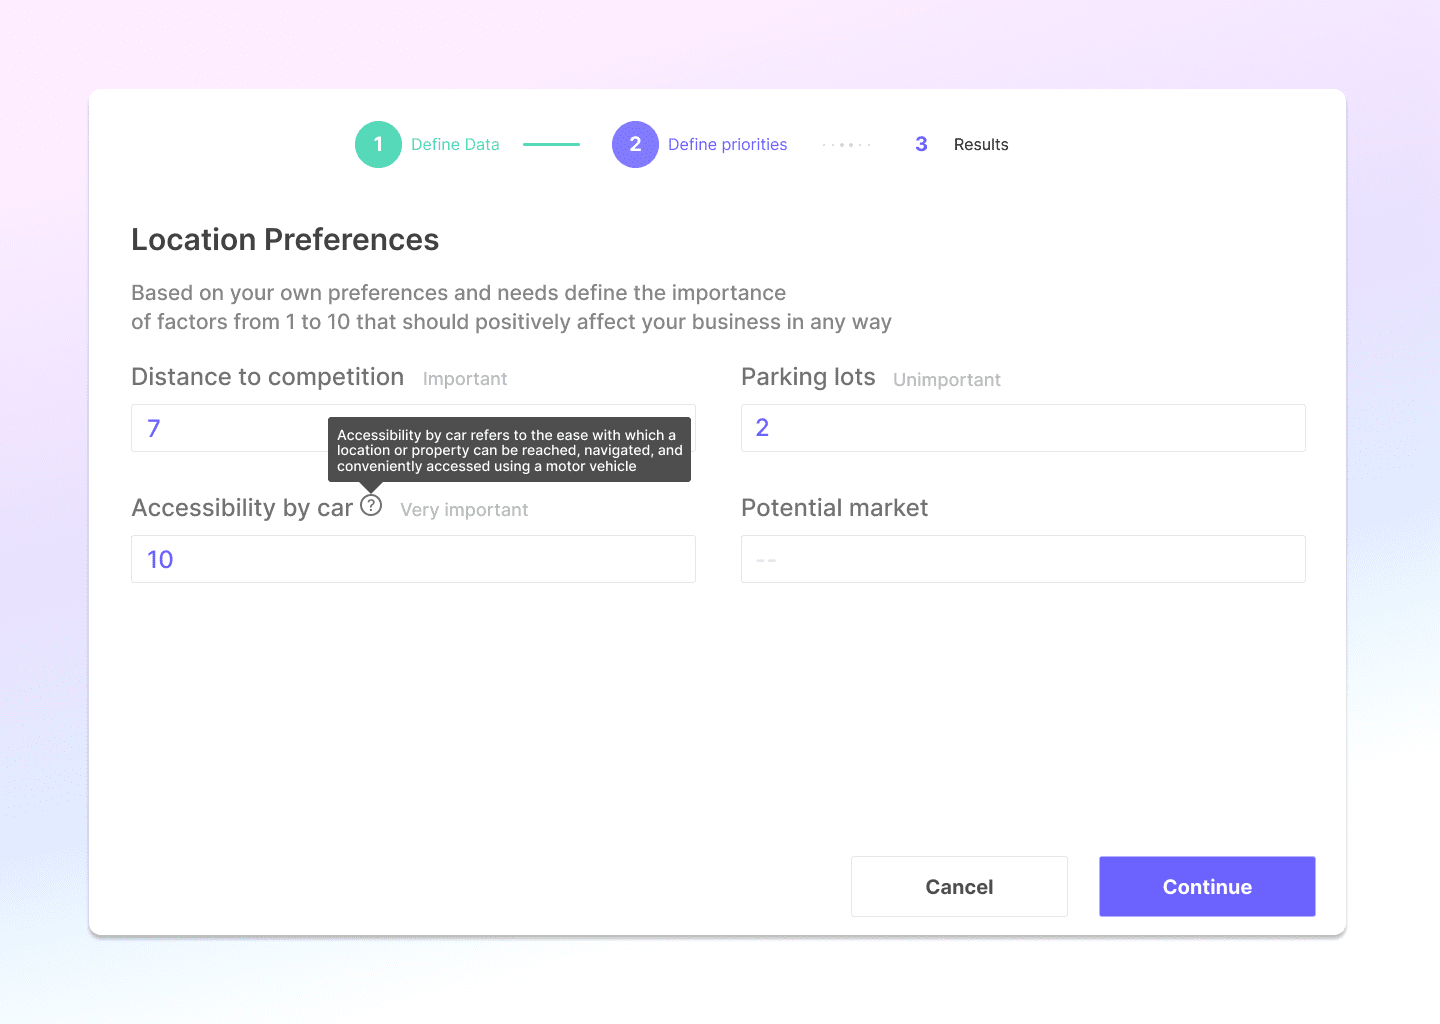
\includegraphics[width=0.9\linewidth]{obrazky-figures/ch5/config-prototype.png}
  \caption{Prototype of a window with inputs.}
  \label{fig:location-attributes}
\end{figure}